\chapter[Caso di studio]{Caso di studio}

Dopo aver descritto il modello fp-HDGM da un punto di vista matematico e metodologico, in questo capitolo esso viene applicato al fenomeno del bike sharing. L'obiettivo iniziale del caso di studio è descrivere, sia nel tempo sia nello spazio, il numero di ritiri di biciclette presso una serie di stazioni (o punti di ritiro) dislocati nel quartiere Jersey della città di New York. Dopodiché, si vuole costruire una mappa di potenziale di mercato spaziale per capire dove conviene aprire una nuova stazione al fine di aumentare il numero di ritiri e il bacino d'utenza del servizio, tenendo conto dell'iterazione concorrenziale esistente tra le stazioni.

\section[Stato dell'arte]{Stato dell'arte}
Nelle città di tutto il mondo, l'inquinamento atmosferico rappresenta una sfida sempre più urgente e complessa. Samantha Burgess, Deputy Director del Copernicus Climate Change Service, ha affermato che il 2023 non solo è stato l'anno più caldo mai registrato, ma è anche il primo in cui tutti i giorni le temperature hanno fatto registrare valori superiori di almeno \SI{1}{\degreeCelsius} rispetto al periodo preindustriale\footnote{\url{https://climate.copernicus.eu/copernicus-2023-hottest-year-record}.}.
\par L'aumento del traffico veicolare, in particolare, contribuisce in modo significativo alla diffusione di gas nocivi (es. CO$_2$ ed NO$_\text{X}$) e particolato nell'aria (es. PM\num{2.5} e PM\num{10}), compromettendo la salute pubblica e l'ambiente. In questo contesto, il bike sharing emerge come una soluzione innovativa e sostenibile per affrontare l'inquinamento urbano. Attraverso la condivisione delle biciclette, questo sistema offre un'alternativa efficace al trasporto privato a motore, riducendo le emissioni di gas serra, i consumi energetici e migliorando la qualità dell'aria nelle città~[\cite{paper_bike_sharing_e_ambiente}].
\par Per modellare il fenomeno del bike sharing le condizioni del tempo atmosferico risultano essere appropriate. Infatti, le variabili meteorologiche come pioggia, temperatura e vento, giocano un ruolo cruciale nel determinare la frequenza e la disponibilità delle biciclette per gli utenti, nonché la percezione stessa dell'attrattività del bike sharing come mezzo di trasporto. Inoltre, risulta interessante capire se la vicinanza di un punto di ritiro dalla più vicina fermata del treno o metropolitana incentiva l'utilizzo di quest'ultima piuttosto che della bicicletta, soprattutto in condizioni di maltempo~[\cite{paper_bike_sharing_e_meteo}].
\par In generale, anche gli aspetti urbanistici e demografici possono aiutare nella descrizione del fenomeno. Infatti, la densità abitativa, la disposizione delle infrastrutture ciclabili, la distribuzione della popolazione, la vicinanza ad alberghi e ai punti di interesse possono influenzare l'adozione della bicicletta a noleggio come mezzo di trasporto urbano~[\cite{paper_bike_sharing_e_popolazione}].
\par Infine, anche gli eventi straordinari possono avere un impatto significativo sul comportamento degli utenti e sulla dinamica del sistema. Uno di questi eventi straordinari è rappresentato dal lockdown imposto a causa della pandemia di COVID-\num{19}. Il lockdown ha comportato una serie di cambiamenti radicali nelle abitudini di spostamento delle persone, con effetti tangibili sull'utilizzo del bike sharing nelle metropoli di tutto il mondo. Pertanto, è essenziale comprendere come la chiusura obbligata abbia influenzato il fenomeno in oggetto, considerando sia gli aspetti legati alla riduzione del trasporto pubblico che quelli associati alla promozione di modalità di spostamento individuali e sicure~[\cite{paper_bike_sharing_e_covid}].
\par In questo contesto, l'impiego di un modello spazio-temporale funzionale si presenta come una soluzione promettente per catturare la dinamica complessa che governa il noleggio e scambio di biciclette. Tale famiglia di modelli consente di considerare non solo le variazioni spaziali dell'utilizzo delle biciclette all'interno di una città, ma anche come queste variazioni si evolvono nel tempo, consentendo una comprensione più approfondita dei pattern di utilizzo e dei fattori che li influenzano. Altresì, la modellazione funzionale permette di descrivere l'evoluzione oraria del numero di ritiri durante il giorno. Infatti, quest'ultimo non rimane costante nel corso della giornata, ma presenta un andamento periodico che raggiunge i propri massimi nelle ore di punta. I trend periodici, inoltre, sono influenzati dalla tipologia di giorno, ovvero feriale o weekend (figura~\ref{trend_paper_Otto}), quindi tenere in considerazione quest'aspetto nella modellazione è fondamentale~[\cite{paper_bike_sharing_Otto}].

\begin{figure}[h!]
	\centering
	\subfigure[]{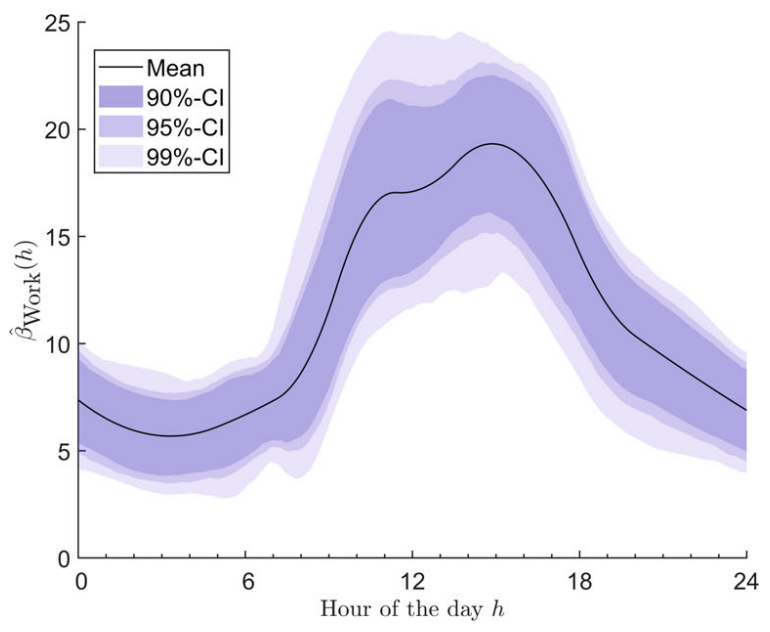
\includegraphics[height=168px]{Immagini/4. Caso di studio/Stato dell'arte/Trend_feriale}\label{trend_feriale}}\quad
	\subfigure[]{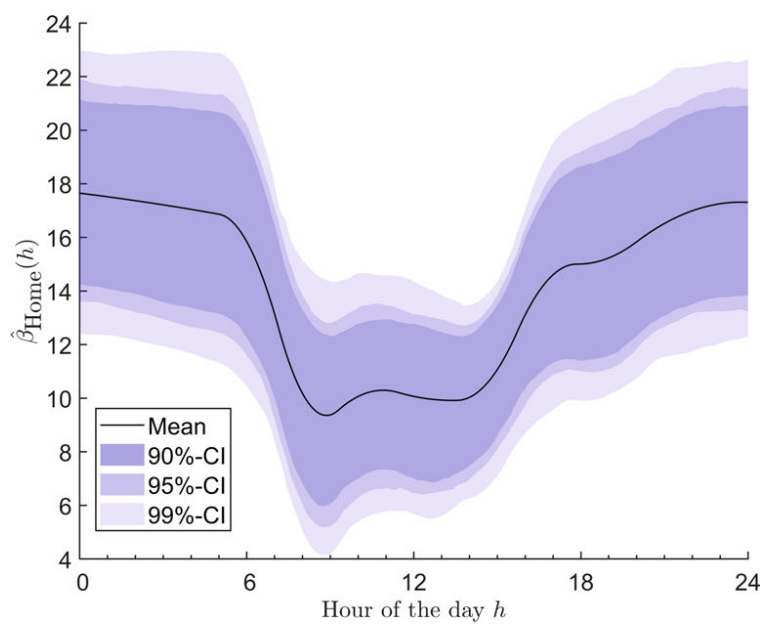
\includegraphics[height=168px]{Immagini/4. Caso di studio/Stato dell'arte/Trend_festivo}\label{trend_festivo}}\quad
	\caption[Confronto tra l'andamento orario del numero medio di ritiri nei giorni feriali e nei weekend a Helsinki]{confronto tra l'andamento orario del numero medio di ritiri di biciclette nei giorni feriali (a) e nei weekend (b) nella città di Helsinki, Finlandia.}
	\label{trend_paper_Otto}
\end{figure}

\section[Ricerca e acquisizione dati]{Ricerca e acquisizione dei dati}
Di seguito sono riportate le sorgenti dei dati utilizzati nel caso di studio:
\begin{itemize}
	\item \textbf{dati riguardanti il bike sharing}: provengono dal sito web Kaggle\footnote{\url{https://www.kaggle.com/datasets/vineethakkinapalli/citibike-bike-sharingnewyork-cityjan-to-apr-2021}.} e contengono le informazioni sul noleggio di biciclette nel \num{2020} dell'azienda Citi Bile a Jersey City. Citi Bike è un sistema di bike sharing pubblico di proprietà privata che serve i distretti di New York City, nello specifico Bronx, Brooklyn, Manhattan e Queens, oltre a Jersey City;
	\item \textbf{dati meteorologici}: contengono le serie storiche delle variabili meteorologiche più significative per la città di New York nel \num{2020}. Il provider di questi dati è Visual Crossing\footnote{\url{https://www.visualcrossing.com/weather-api}.}, un fornitore che offre una vasta gamma di soluzioni per l'accesso ai dati meteorologici storici e in tempo reale, nonché per la generazione di previsioni meteo;
	\item \textbf{dati inerenti le stazioni del treno/metropolitana}: dopo aver recuperato i nomi delle stazioni del treno e della metropolitana dalla mappa dei mezzi pubblici newyorkesi\footnote{\url{https://stewartmader.com/subwaynynj/}.}, le loro coordinate sono state reperite tramite Google Maps;
	\item \textbf{dati demografici}: il fornitore è il SEDAC\footnote{\url{https://sedac.ciesin.columbia.edu}.} (Socioeconomic Data and Applications Center), un data center che fa parte del programma Earth Observing System Data and Information System (EOSDIS) della NASA. La missione principale dell'ente è quella di fornire accesso a dati socioeconomici e ambientali globali, nonché a strumenti e risorse per facilitare la ricerca e la comprensione dei cambiamenti ambientali e delle dinamiche sociali.
	\item \textbf{dati riguardanti i giorni di festività e di lockdown}: per i primi è stato fatto riferimento al sito web OfficeHolidays\footnote{\url{https://www.officeholidays.com/countries/usa/new-york/2020}.}, mentre per i secondi a Wikipedia\footnote{\url{https://en.wikipedia.org/wiki/COVID-19_pandemic_in_New_York_City}.}.
\end{itemize}
Da sottolineare, infine, che sono state processate le sole variabili d'interesse per il caso di studio; nello specifico è stato applicato un raggruppamento su base oraria, ove necessario.

\section[Descrizione del dataset]{Descrizione del dataset}